\newpage
\section{Opis systemu}

\subsection{Architektura}

Aby spełnić wszystkie postawione powyżej wymagania, zdecydowano podzielić system na kilka osobnych aplikacji, pomiędzy którymi komunikacja jest zrealizowana za pomocą adekwatnych protokołów sieciowych. Poszczególne moduły oraz połączenia pomiędzy nimi przedstawiono na rysunku \ref{fig:architektura}. Dzięki takiemu rozwiązaniu, można było wykorzystać dostępne oprogramowanie do symulacji dynamiki oraz kompletne oprogramowanie autopilota stosowane na rzeczywistych BSP. Dużą zaletą zastosowania ArduPilot SiTL \begin{todo}https://ardupilot.org/dev/docs/sitl-simulator-software-in-the-loop.html\end{todo} jest format danych w którym przesyłane są informacje o stanie BSP. Ponieważ jest identyczny z komunikacją wysyłaną z rzeczywistego BSP kontrolowanego z wykorzystaniem \emph
{firmware} ArduPilot, można wykorzystywać taki sam program do łączenia z symulacją jak i fizycznym BSP w trybie AR.

\begin{figure}[!h]
    \caption{Schemat elementów systemu}
    \label{fig:architektura}
    \centering 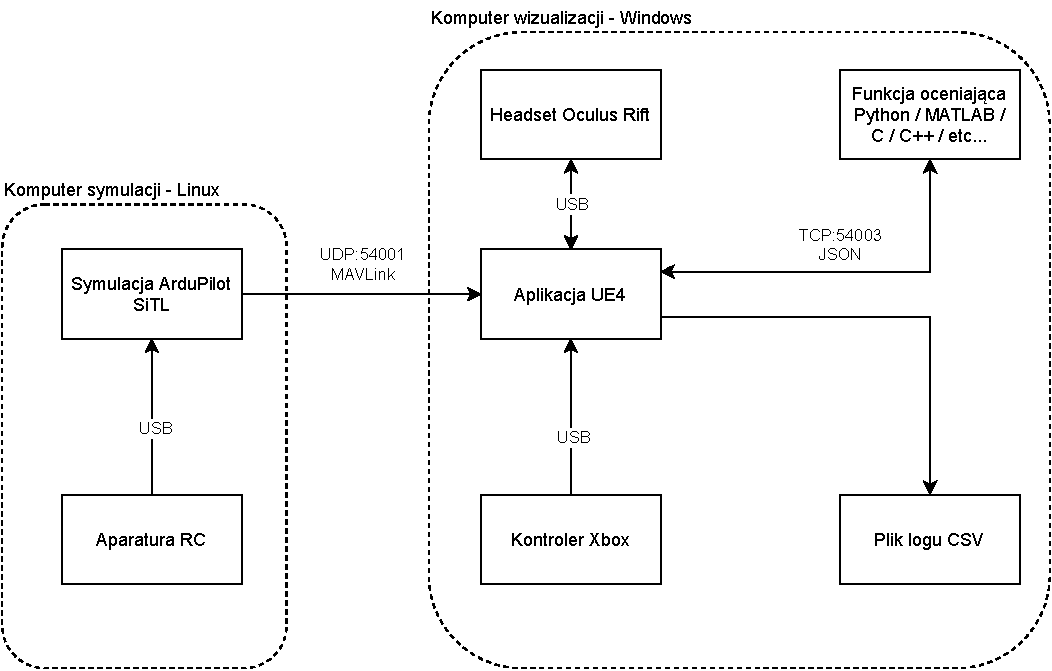
\includegraphics[width=0.8\linewidth]{architektura.pdf}
\end{figure}

Aby móc stosować jedną aplikację zarówno z goglami VR oraz AR, wizualizacja została przygotowana z wykorzystaniem Unreal Engine 4 \begin{todo}https://www.unrealengine.com/\end{todo}. To środowisko jest przykładem tzw. ,,silnika'' gier komputerowych. Aby umożliwić uruchamianie tej samej aplikacji na różnych platformach z wykorzystaniem różnego sprzętu, wprowadza liczne warstwy abstrakcji i gotowe klasy, dzięki czemu użytkownik musi jedynie zaimplementować własne kluczowe funkcjonalności programu (tzw. \emph{business logic}). Widoczny na schemacie ,,Kontroler Xbox'' jest popularnym urządzeniem HID, które wykorzystywane jest w grach komputerowych. Ponieważ także posiada parę dwuosiowych drążków, ale jest prostszy w obsłudze od pełnego nadajnika zdalnego sterowania dla BSP, jest zastosowany jako zastępczy kontroler do prowadzenia prostych testów nowych funkcji bez potrzeby uruchamiania programu symulacyjnego AP~SiTL. Podobnie jak w przypadku urządzeń wyświetlających, sterownik jest zaimplementowany przez zespół Unreal, konieczne było jedynie przypisanie odpowiednich funkcji do przycisków i analogowych osi urządzenia.

Środowisko Unreal Engine oferuje bardzo dużo gotowych funkcji, ale przez to jego kod źródłowy jest bardzo obszerny i może być przytłaczający dla nowego użytkownika. Aby umożliwić pisanie funkcji oceniających operatora w językach innych niż C++ oraz rozwiązać wspomniany problem skomplikowania środowiska, ocena operatora także została wydzielona do osobnego procesu skomunikowanego przez protokół TCP/IP \begin{todo}przypis TCP\end{todo}.

Wyniki działania wszystkich elementów programu zapisywane są do pliku tesktowego w formacie CSV \begin{todo}przypis CSV\end{todo}. Wadą takiego rozwiązania jest mało efektywne wykorzystanie przestrzeni dyskowej w porównaniu z zapisywaniem danych w formacie binarnym, w postaci w której znajdują się w pamięci operacyjnej podczas działania programu. Mimo to zastosowano ten format ponieważ plik danych jest zrozumiały dla człowiek bez stosowania specjalnego dekodera. Ponadto, obsługa plików tego typu jest zaimplementowana w licznych pakietach obliczeniowych m.~in. MATLAB lub Microsoft Excel. Biorąc pod uwagę że symulator ma być elastycznym narzędziem do wykonywania badań, głównym kryterium wyboru było zapewnienie czytelności i swobody wyboru nardzędzi dla użytkownika.

\subsection{Aplikacja wizualna}
\begin{todo}
    Wykorzystane rozwiązania, przykłady jak wyglądała w kolejnych iteracjach, konkretne klasy napisane w C++, sposób dodawania nowych zadań i modeli
\end{todo}

Jak wspomniano powyżej, cechą charakterystyczną przygotowanej wizualizacji jest wykorzystanie silnika Unreal Engine. Warunki licencyjne tego oprogramowania pozwalają na darmowe wykorzystanie go także w projektach komercyjnych, pod warunkiem że zysk nie przekracza ustalonego progu. Mimo tego, dozwolone jest modyfikowanie środowiska do własnych zastosowań, co jest ułatwione przez dostępność kodu źródłowego całego silnika.

\subsubsection{Komunikacja z symulacją BSP}

Po sformułowaniu wymagań i wstępnym wyborze rozwiązań, w pierwszej kolejności przygotowano prototyp sprawdzający możliwość połączenia oprogramowania ArduPilot z Unreal Engine. W tym celu konieczne było wykorzystanie biblioteki MAVLink \begin{todo}https://mavlink.io/\end{todo}, która jest wykorzystywana do komunikacji przez różne systemy BSP, w tym ArduPilot.

\begin{todo}
    Zrzut ekranu z prymitywnego poziomu.
\end{todo}

\begin{todo}
    Algorytm interpolacji jak w Quake World, z wykresami ilustrującymi różne podejścia
\end{todo}

\subsection{Serwer oceny}
\begin{todo}
    Sposób komunikacji, dane dostępne do oceny, przykładowy serwer w kilku językach
\end{todo}

\subsection{Dokumentacja}
\begin{todo}
    Instrukcja dla użytkownika i dla dewelopera, przykład tekstu w Markdown, sposób publikacji
\end{todo}